\chapter{The Fundamentals of Resilience in Cloud Computing}
\label{ch:resillience}


\comment{Create introduction after Meta text}
Nygaard describes how software engineering is taught incompletely, and that focus when developing distributed software should be shifted. Nygaard states that focus should be on what a system should not do, contra today's focus on what a system should do. The first acknowledgement when developing distributed systems is according to Nygaard the realisation that failure will occur, and focus should be on handling them instead of avoiding them altogether. Further stating that a stable system will keep on working as intended, even though persistent stress or component failure is present. Nygaard states the following\cite[p. 27]{nygard2007release}:

\tquote{Once you accept that failures will happen, you have the ability to design your system's reaction to specific failures. [..] This sort of self-protection determines the whole system's resilience.}{Nygaard}{2007}

Strigini describes a movement within information and communication technology, stating that newly developed systems are more interconnected and changed without global system intervention by developers. Setting unprecedented requirements to existing practices of dependable design, making current practices inadequate when trying to deliver satisfactory levels of dependability\cite[p. 5]{strigini2012fault}.

\tquote{While existing practices of dependable design deal reasonably well with achieving and predicting dependability in ICT systems that are relatively closed and unchanging, the tendency to making all kinds of ICT systems more interconnected, open, and able to change without new intervention by designers, is making existing techniques inadequate to deliver the same levels of dependability}{Strigini}{2012}

Dealing with resilience in distributed systems is a necessity, when applications are growing in scale and complexity. The following chapter will establish a definition of resilience, which can be used to evaluate application and infrastructure architecture. 

\section{Defining resilience}
Resilience stems from the Latin word resilíre, meaning "to leap back". Relating it to software engineering it can be defined as a systems ability to "bounce back" and adapt to disruption\cite{omer2013resilience}. Resilience has been used within many disciplines before being applied to software engineering, and has been defined very broadly, potentially incorporating many aspects within cloud computing. The following section will try to pin down what resilience means within cloud computing and what it entails to strive for a system with a high resilience.


Resilience has been defined and characterised by many different parties, within several disciplines.\cite{folke2002resilience, dalziell2004resilience, rose2005modeling, andersson2006urban, fiksel2003designing, bruneau2003framework, reed2009methodology, pavard2006design}
These definitions help understand the meaning of resilience, and link it to the understanding of cloud computing. Important keywords from these definitions have been identified, creating an overview of different resilience characteristics. The keywords identify the core concepts that resilience convey when used, all very relevant when defining resilience within cloud computing.

All collections of keywords relate very closely, and help define key concepts within resilience with keywords such as: \textit{stable equilibrium, cope, adapt, proactive measures, reorganize, retain structure, redundancy, robustness}. The context in which there is a necessity for resilience is also included and clear, focusing on the possible disruptive events, described with the following keywords: \textit{undergoing change, face of disruption, face of stress, perturbation, disruptive events}, emphasizing the need for resilient systems in environment characterized by these keywords.

The keywords can be grouped and related to know principles within cloud computing, helping simplify the broader characteristics of resilience, creating a model for a cloud computing related resilience definition. The keywords have been grouped according to their association, under a headline inspired directly by the identified resilience keywords and known cloud computing keywords, seen on figure \ref{fig:resilience_keywords_grouped}. The two overarching words being \textit{dependability} and \textit{adaptivity} each with several sub-concepts, all described in the following section.

\begin{figure}[!htb]
  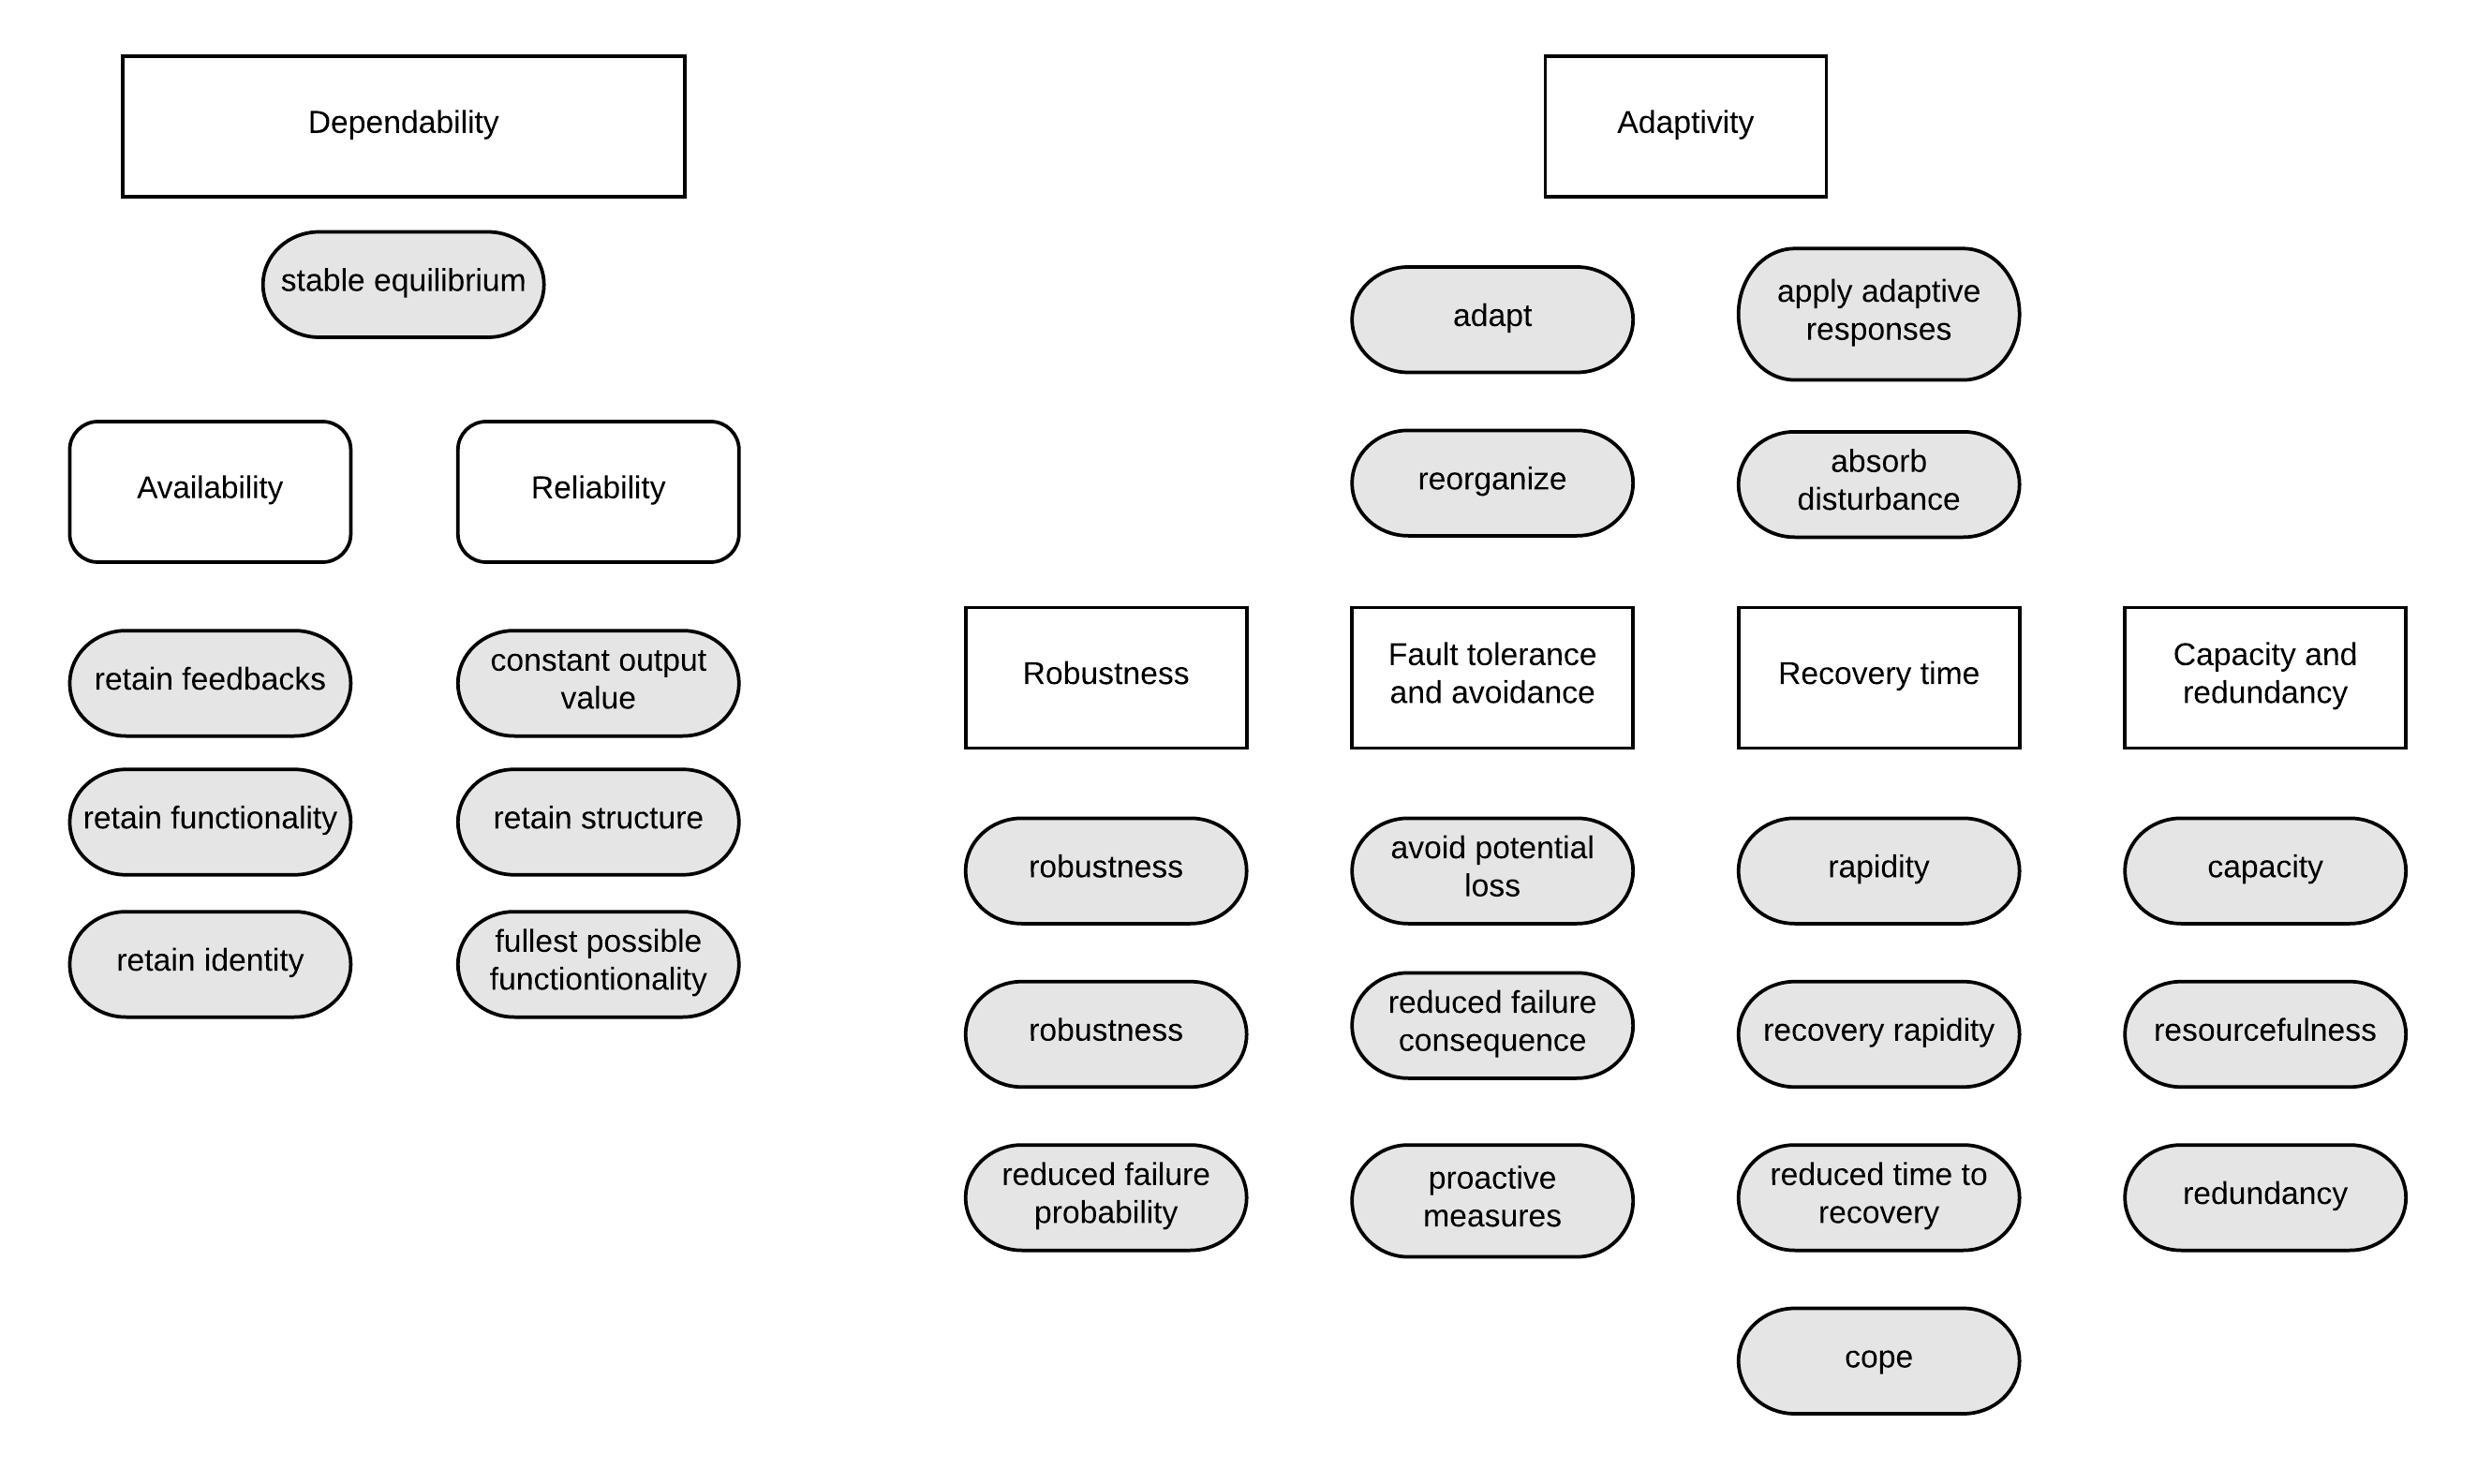
\includegraphics[scale=0.15]{resilience_keywords_grouped}  
  \caption{Resilience keywords grouped in a cloud context}
  \label{fig:resilience_keywords_grouped}
\end{figure}
\newpage
\subsection{Dependability}
Dependability describes the systems ability to deliver the intended level of service, whether the users can rely on the servie level. Having a dependable service means to have a service level that is not impacted by faults and their derived errors. The users of a system perceive the system state as an alternation between service accomplishment and interruption, either a service is precisely as specified or different. The transition between these states are controlled by restoration and failure events, either pushing the service in a direction that aligns or deviates with the intended service level. Dependability is mainly quantified through measures on \textit{availability} and \textit{reliability}\cite{laprie1985dependable}.


\textbf{Availability} describes the accessibility to data, and is generally determined by calculating the time a service was unavailable, over a given period. The availability level can then be determined, by stating how much downtime is allowed, within a given period\cite[p. 477]{beyer2016siteReliabilityEngineering}. Is the data available to users or dependent service boundaries? If data is not available to our users, it does not exist from their perspective\cite[p. 345]{beyer2016siteReliabilityEngineering}.

\comment{Kig på 'Measuring Service Risk' side 26 is site reliability engineering}

\textbf{Reliability} is the probability that a system will fulfil set requirements in stated conditions for a given period of time\cite{o2012practical}. The resilience of the system therefore determines the reliability, by analysing the amount of external disruption a system can handle. Google states that reliability is the fundamental feature of a system, and autonomous and resilient system behaviour is a good way to achieve reliability\cite[p. 84]{beyer2016siteReliabilityEngineering}.


\subsection{Adaptivity} \comment{Should it be adaptive capacity?}
Adaptivity can be defined as the systems ability to adapt to a disruptive situation and reconfigure themselves, without loss in the intended level of service. Including the ability to adjust to changing internal demands\cite{reed2009methodology}. Adaptivity contains, \textit{Robustness}, \textit{Fault tolerance and avoidance}, \textit{Recovery time} and \textit{Capacity and redundancy}.


\textit{Robustness} covers how quantifiable the system behaviour is in the face of disruption challenging system behaviour\cite[p. 10]{sterbenz2010resilience}. These disruptions are both internal and external\cite{omer2013resilience}. Robustness includes the systems ability to withstands disruptions rather than adapt to them, a robust system has been designed to withstand known uncertainties, maintain intended level of service and same form of functionality.
\comment{Kig på: "Evaluating robustness of cloud-based systems" Godt input til robustness}

\textit{Fault tolerance and avoidance} is used to describe dependability of a system, from internal and external harm. Tolerance is making the system tolerable to the effects of faults. Avoidance meaning guarding a system against potential defects, that could cause system failure\cite{strigini2012fault}.


\textit{Recovery time} is a measure for how long time period a system needs to resume fulfilling the stated requirements.


\textit{Capacity and redundancy} is two different aspects that inherently are very linked. Capacity is the highest throughput a system can deliver, with and acceptable response time for each request\cite[p. 136]{nygard2007release}. Redundancy meaning how much extra capacity a system has, that can be applied in case of failure to uphold stated system requirements.

\note {
\begin{figure}[!htb]
  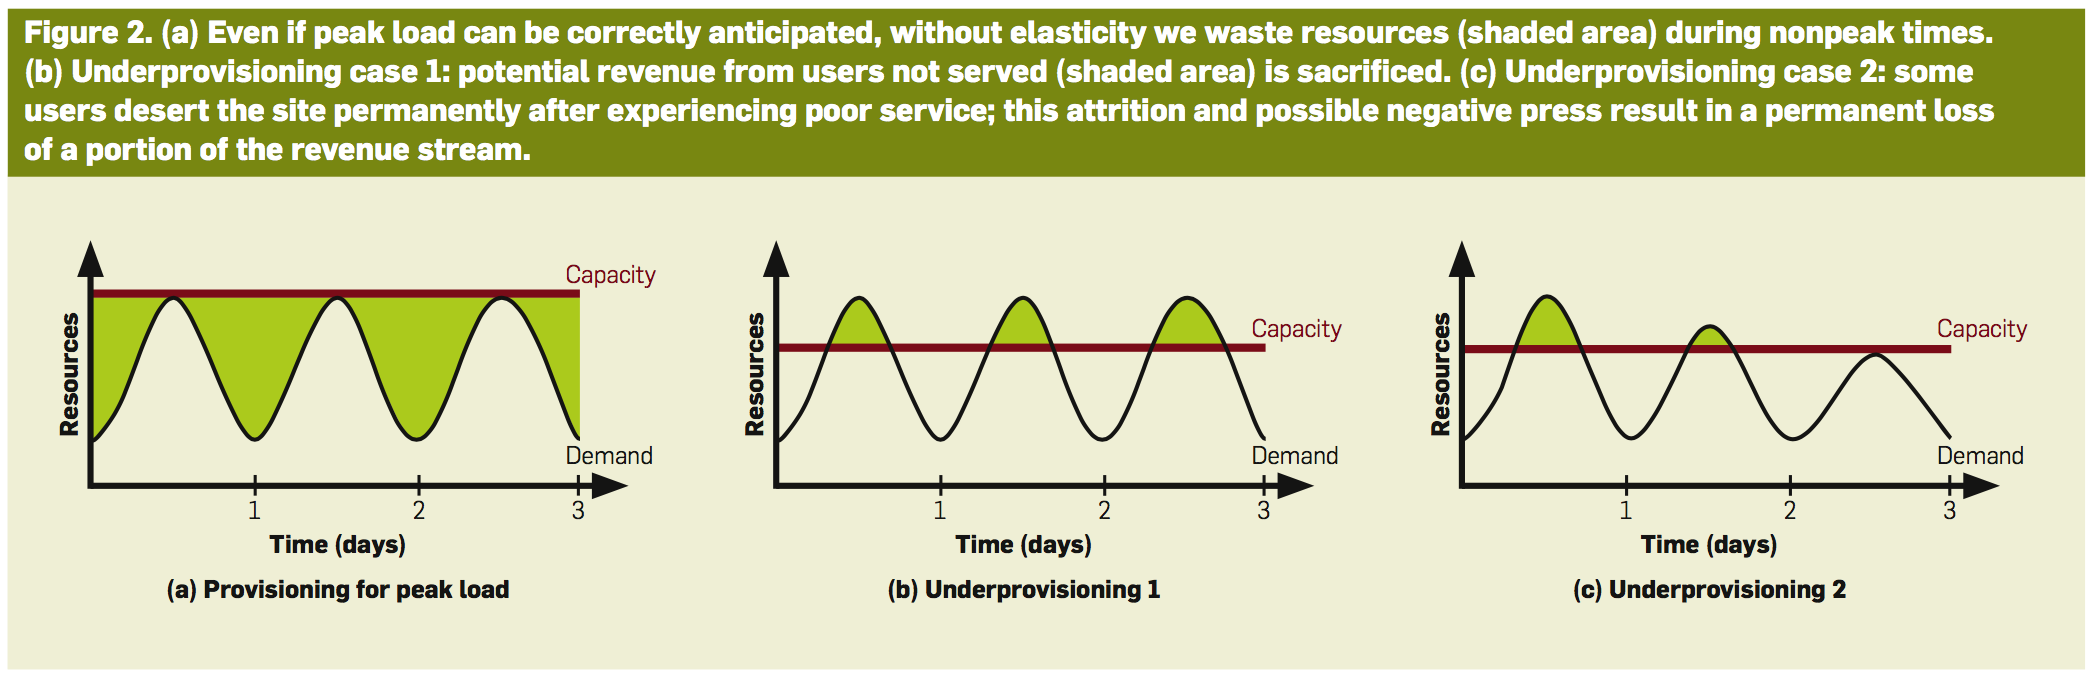
\includegraphics[scale=0.15]{resilience_capacity}  
  \caption{Capacity figure from: Ambrust et al. – A View of Cloud Computing \comment{Make own picture of this :).}  }
  \label{fig:resilience_keywords_grouped}
\end{figure}

\comment{Agree on server, system, service and layer Abstractions}
\comment{The layer abstraction should be explained like in his book} 
\comment{Explain service-oriented architecture}
\comment{Define operations}
}

\section{Stability Antipatterns}
\label{sec:stability_antipatterns}
When working with big complex systems, rest assure: Failure is bound to happen. How the failure was triggered, which fractures it created and how much it propagated will differ each time. Stability antipatterns is a concept Nygaard uses when understanding how these failures appear within a distributed system, which characteristics the failures have and how some architectures leads to them.\cite[p. 31]{nygard2007release}.

\subsection{Integration Points}
Integration points are connections from a service to other services, necessary for the service to deliver expected functionality. Nyggard denote integration points as the :\textit{"The number-one killer of systems"}\cite[p. 33]{nygard2007release}. Integration points often run over socket connections which are not immediate and incur complexity. Many simultaneous connections can hamper a remote application, forcing the calling application to wait, and possible decrease service level.
Circuit breakers, decoupling middleware and testing can help solve or identify challenges with integration points.

\subsection{Chain Reactions}
Chain reactions can form if one of several serving servers fail, and therefore inflict a higher load on the remaining running servers. If one server has failed because of an internal error, load is increased on the remaining servers, also containing internal errors, increasing the probability of similar errors happening in the remaining servers. Typical errors include resource leaks and obscure race conditions.
Server bulkheads prevent chain reactions from depleting entire services, circuit breakers protect caller services.

\subsection{Cascading Failures}
Cascading failures happen when a failure from one layer cause problems in callers. If a failure happens in a serving service and callers are not correctly handling it (eg. implementing a time-out) the failure can cascades into the calling service. Nygaard calls cascading failures "the number on crack accelerator"\cite[p. 49]{nygard2007release}.
The circuit breaker pattern and timeouts can combat cascading failures.

\subsection{Users}
Users increase the amount of traffic, and will eventually surpass capacity, unless increased with a growing demand. If a transaction is too long, the demand has surpassed the capacity. Derived errors can occur if the capacity is fully utilized, for example memory exhaustion, causing other internal services to fail. These derived errors can be combated with a correct service capacity.

\subsection{Blocked Threads}
Concurrency errors within a service, can block several threads. Timeouts in wait functions can defend against indefinitely blocked threads.

\subsection{Attacks of Self-Denial}
Attacks of self-Denial is never a system error, but the people around the system. Nygaard describes situations where advertisement campaigns has created big spikes of sudden and unforeseen load, that takes the system down due to insufficient capacity. 
Either a "shared-nothing" architecture, decoupled middleware or horizontally scaling of the shared resources required in the advertisement campaign can mitigate self-denial attacks. A "shared-nothing" architecture encapsulates the entire service within a single server, making it linearly scalable, combating huge load spikes and isolating possible failures.

\subsection{Scaling Effects}
Scaling effects describe the effects of a system handling increasing amounts of load, previous sufficient capacity levels becomes insufficient. Test environments often do not show scaling effects due to their limited scale.
Scaling effects can be negated by avoiding internal point-to-point communication and stress testing shared resources, implementing proper fallback behaviour if they fail.

\subsection{Unbalanced Capacity}
Unbalanced capacity refers to the service capacities of dependent services, and their balance. Capacity variance between development and deployment environments and what potential fallacies this can introduce. Unbalanced capacity can introduce scaling effects, where one service scales accordingly whereas another, dependent service capacity, remains stagnant.

\subsection{Slow Response}
Quick responses lets the calling service proceed rapidly, a slow responses on the other hand, ties the resources that the calling service is using for a longer period. Slow responses can trigger cascading failures, due to slow upstream responses from a calling service that is tied up in a slow response. Slow responses causes increased amounts of traffic due to users frequently reloading pages loading slowly. Slow responses can be solved by failing fast if response times exceeds upper timing limits, and ensuring that there is not a shared resource contention.
A slow response ties up the resource on the calling end, the longer a call is on a service provider, the larger the caller needs to scale, to handle the same amount of traffic.

\subsection{SLA Inversion}
Service-level agreement inversion is when a service promises a specific service level without taking into account the service-level agreement of the services it relies on. Service-level is determined by the dependencies service-levels and the probability for failure internally. It is therefore important to decouple from dependent services and degrade functionality gracefully as dependant services fail. If decoupling is not possible, circuit breaks can be put into place. 

\subsection{Unbound Result sets}
Unbound results sets occur when the amount of requested data is not limited, and the result set therefore grows equally with the entire data set. Limiting the result set will ensure that memory in the calling application will not be exhausted, if the data set is expanding.


\section{Stability patterns}
Stability patterns are applied to increase stability and reduce damage done when errors occur. These patterns serve as design guidance when implementing services.


\subsection{Timeouts}
Network connections are slow and error prone, but necessary to incorporate in any distributed application. Applying timeouts at integration points help avoid blocked threads and mitigate slow responses from dependent services. By defining timeouts an upper limit for time waiting is set, the application can then move on and recover from failure.

\comment{Perspektiver til mit fine diagram. :)}

\subsection{Circuit Breaker}
The circuit breaker pattern is based on the principles and functions of a fuse in electric circuits. From a software perspective, the idea is to wrap dangerous operations, so that they can be circumvented when not working properly. This allows a system to degrade functionality if errors occur, guarding against integration points, slow responses, unbalanced capacities and cascading failures.

The circuit break is a state machine pattern, moving between three states: open, closed and half-open. When in open state, requests are processed ordinarily. When in closed state, requests fail immediately. The circuit break can transit from open to closed if requests unexpectedly are unsuccessfully processed. The half-open state processes requests ordinarily to test if it is possible to process requests successfully. If requests are processed successfully in the half-open state, the circuit breaker changes the state to open. A threshold specifies the amount of unsuccessful processed requests, that triggers state transition from open to closed state. Another threshold determines when to transit form closed to half-open states.

Circuit breaker guards against integration points, when a failure occurs in a integration point, it should not be called. Used together with timeouts, that can inform the system of a present error.
\comment{Perspektiver and insert diagram}

\subsection{Bulkheads}
The bulkheads design pattern is inspired by bulkheads know from ship design, where compartments throughout the ship divides the ship into watertight partitions. This ensures that a single penetration of the ships hull, does not sink the ship. When applied to software, bulkheads is used to partition capacity, preserving functionality if errors occur. Bulkheads can protect against chain reactions, by ensuring backups of services important to several other services. The bulkhead pattern is usable on both a application and infrastructure level, by partitioning thread pools, server CPU or separate servers, determining the granularity. 


Bulkheads are excellently implemented with virtualization, where capacity can be changed quickly by increasing or decreasing the allocated amount of independent services.
\comment{Insert diagram}

\subsection{Steady State}
Steady state refers to intended state of a service, where the functionality is completely fulfilled and the service is operating as intended. Many factors influence this steady state and some potentially interrupts it. Manual operations incur overhead and eventually introduce human made errors, a system should be able to run indefinitely without operational intervention. \comment{Mention afore mentioned dev ops} Further more mechanism that accumulates resources must be drained at the same rate or greater not to overflow. When mechanism overflow, errors can occur by increasing response time or slowing down databases. By purging unused data from databases, clogging of server memory is avoided, which could potentially slow read and write operations. Log files is also a potential memory clog, and should therefore be left of the production server.
\comment{Talk more in depth about dev ops, use site reliability engineering book}


\subsection{Fail Fast}
The fail fast principle dictates informing callers quickly, when a system SLA cannot be met. By failing fast the system avoids incurring internal problems externally. By verifying that integration points are correctly working early, potentially wasted resources are reserved by completely avoid running transactions that cannot complete in their entirety.

\subsection{Handshaking}
Handshaking refers to how services accept future workloads from other services. By acknowledging that the service can live up the the stated SLA, and service the required capacity before communication begins. The service can protect itself by throttling incoming requests to serviceable levels. Health checks, where a service is checked before calling can spare a standard call that fails.

\subsection{Test Harness}
A test harness is a supplement to traditional unit tests, acceptance test. The test harness job is to emulates remote systems on the other side of integration points, and mimic responses to remote calls on the network. By mimicking the dependencies, developers are able to test how the service reacts to malicious responses of different kinds.

\subsection{Decoupling Middleware}
Decoupling Middleware is the communication protocol used to communicate between dependent but decoupled services. Varying from same time, host and process to different time, host and process.

Nygaard describes how fundamental it is to the system design which form of communication is chosen, and how big consequences for the implementation changing this has. Choosing communication in a system is on an architecture level, fundamentally changing the implementation of individual services within the system.
\comment{Expand this, I feel like this is very important. Find more sources talking about this}

\comment{Use the notes from the goto conference video:}
\note{
\section{Nygaard Stability Patterns and Antipatterns}

\url{https://www.youtube.com/watch?v=VZePNGQojfA}
Worked as devops, identified some recurring problems, 'luckily'


\textbf{Definition of availability:}
Probability that system is operating at time t.
When I do something, is the system successfully going to complete that thing? Complete the mission that it is given.
Has nothing to do with servers running, hardware being alive.
Not something that is directly controllable. You ability to introduce stability in your software.

\textbf{Stability}
Architectural characteristic, allow to maintain availability. In the face of outrageous fortune.  
Slings and errors of faults and errors.

\textbf{Fault}
Incorrect internal state. Initiated internally, or something introduced from the outside, through network for example.
Fault-tolerance - You recover internal incorrect state, you use exception handlers f.example.
Fault-intolerance - As soon as i detect incorrect internal state, terminate.

We want to stop the system from producing an error.

\textbf{Error}
If the system produces incorrect output, or the behaviour of the system is different than usual. If the system starts hammering another system, with exessive request, thats an error in behaviour.
On account of a undiscovered fault in the system.

\textbf{Failure}
Some errors lead to failures.
Loss of availability. The system is unresponsive. The system can no longer accomplish its mission.
We want to avoid failure.

\textbf{Wicked database hang}
A lot of variables in the particular problem, the situation was very unique. 
It is impossible to engineer every problem away from every integration point. Therefore you need to put in things in place that prevent a failure at a integration point, to propagate to the entire system, and take it down.

\textbf{in spec vs out of spec "wicked error"}
Unless you force them in QA, you only get the wicked error in production, unless you design QA with them included.
Use a test harness to find the problems in development.

\textbf{Patterns to help with integration points}
Use circuit break, use timeouts, use decoupling middleware, handshaking.

\textbf{Chain reactions}
It is common but wrong to treat horizontal scaled farm of servers, machines or containers, as independent devices. They are highly correlated, through for example software.
Failure in one of a correlated set of applications means that the risk of failure in the remaining applications is higher.

\textbf{Cascading failure}
Let the 'error jump the gap'. Amplifying a failure in a down stream system.


\textbf{Spectrum of calling}
Which implementation of communication do we choose 
Nygaard talks about the spectrum of calling, how in-process method calls are easy and cannot fail. If the library with the function in it, is there, then it works. It is the same time, same host and same process.
Same time, different host and different process, is harder. The call is blocking, but we are not sure to receive a answer any time soon.

The longer we can wait with taking a definitive decision the better. A mix of the communication styles my be preferable.


\textbf{Error will occur}
Errors will occur, the big question is whether we amplify them or do something to dampen or nullify them in our organization. 
If a system is fatigue, failure can occur, it sets cracks in the structure, that crack can propagate if it is not stopped. We get a catastrophic failure.
If we have crack stoppers in place, dampering the failure, prevent it from propagating and accelerating. 
We cannot prevent the system from getting damaged. But we can preserve some feature for some users, and prevent catastrophic failures.


Nygaard likes the idea of simmian army, it is hard if not impossible to test the system at the same scale as in production. Forcing yourself to be anti-fragile, by creating problems.

Monitoring system design. It is good if it can register heartbeats from the application. A lot of systems only register when something goes wrong. Not getting a heartbeat is something going wrong.
}



\note{
\begin{quote_highlight}
"Ability of the system to resume normal functionality after shock"\cite[p. 15]{omer2013resilience}
\end{quote_highlight}

\begin{quote_highlight}
"ability to deliver, maintain, improve service when facing threats and evolutionary changes" \cite[p. 4]{strigini2012fault}
\end{quote_highlight}


and can according to \cite[p. 15]{omer2013resilience}, be defined as the following within system engineering. "Ability of the system to resume normal functionality after shock"\cite[p. 15]{omer2013resilience}

"Thus, dependability and resilience in cloud computing are of paramount importance to guarantee availability and reliability of services and application execution, even in the presence of large number of faulty components." \citeauthor{abid2014toward}

\begin{quote_highlight}
"A resilient system keeps processing transactions, even when there are transient impulses, persistent stresses, or component failures disrupting normal processing." \cite[p. 24]{nygard2007release}
\end{quote_highlight}


"Here, the word “resilience” is used to identify enhanced ability to deal with the unexpected, or a more flexible approach to achieving safety than the current mainstream approaches"  \cite[p. 5]{strigini2012fault}

"[...] visibly rebounding from deviations and returning to (or continuing in) a desirable way of functioning [...]" \cite[p. 6]{strigini2012fault}



overarching goal of system, continue to function, fullest possible extent, in face of stress, to achieve purpose

proactive preparation and reactive measures, in face of natural hazards


return to stable equilibrium state after disturbance


reduced failure probability, reduced consequences, reduced recovery time


Counterpart to resilience is brittleness, brittle system lack ability to adapt and transmit disruption (onwards in the system i guess)


\cite[p. 4]{omer2013resilience}
"A failure in any one infrastructure could result in cascading failures in other infrastructures. The failure propagate from one element to the next and may have catastrophic consequences. Building resilience into infrastructures prepares the system for mitigating disasters and hence reduces the losses incurred by service disruption"


"The primary factor for implementing resilience in systems is to improve the reaction of the system after the occurrence of disruptions or system shock and improve its ability to resume functionality."

\textbf{Resilience} \cite[p. 5]{newman2015microservices} 
A key concept in resilience engineering is the bulkhead. If one component of a system fails, but that failure doesn’t cascade, you can isolate the problem and the rest of the system can carry on working. Service boundaries become your obvious bulkheads. In a monolithic service, if the service fails, everything stops working. With a monolithic system, we can run on multiple machines to reduce our chance of failure, but with microservices, we can build systems that handle the total failure of services and degrade functionality accordingly.
We do need to be careful, however. To ensure our microservice systems can properly embrace this improved resilience, we need to understand the new sources of failure that distributed systems have to deal with. Networks can and will fail, as will machines. We need to know how to handle this, and what impact (if any) it should have on the end user of our software.
We’ll talk more about better handling resilience, and how to handle failure modes, in Chapter 11.

Knowing how much failure you can tolerate, or how fast your system needs to be, is driven by the users of your system. That in turn will help you understand which techniques will make the most sense for you. That said, your users won’t always be able to articulate what the exact requirements are. So you need to ask questions to help extract the right information, and help them understand the relative costs of providing different levels of service.\cite{newman2015microservices}[p. 206]


\textbf{Cross-functional requirements}\cite{newman2015microservices}[p. 207]
Response time/latency
	How long should various operations take?
	“We expect the website to have a 90th-percentile response time of 2 seconds when handling 200 concurrent connections per second.”


Availability
	Can you expect a service to be down? Is this considered a 24/7 service?


Durability of data
	How much data loss is acceptable? How long should data be kept for? This is highly likely to change on a case-by-case basis. For example, you might choose to keep user session logs for a year or less to save space, but your financial transaction records might need to be kept for many year s.
	
	
Once you have these requirements in place, you’ll want a way to systematically measure them on an ongoing basis. You may decide to make use of performance tests, for example, to ensure your system meets acceptable performance targets, but you’ll want to make sure you are monitoring these stats in production as well!


\textbf{Isolate failure}\cite{newman2015microservices}[p. 248]  - Key, can be used to reason about circuit break
"A microservice architecture can be more resilient than a monolithic system, but only if we understand and plan for failures in part of our system. If we don’t account for the fact that a downstream call can and will fail, our systems might suffer catastrophic cascading failure, and we could find ourselves with a system that is much more fragile than before."


"If we hold the tenets of antifragility in mind, and expect failure will occur anywhere and everywhere, we are on the right track. Make sure your timeouts are set appropriately. Understand when and how to use bulkheads and circuit breakers to limit the fallout of a failing component. Understand what the customer-facing impact will be if only one part of the system is misbehaving. Know what the implications of a network partition might be, and whether sacrificing availability or consistency in a given situation is the right call."

\textbf{Architectural safety measures}\cite{newman2015microservices}[p. 209]
There are a few patterns, which collectively I refer to as architectural safety measures, that we can make use of to ensure that if something does go wrong, it doesn’t cause nasty ripple-out effects. These are points it is essential you understand, and should strongly consider standardizing in your system to ensure that one bad citizen doesn’t bring the whole world crashing down around your ears.


But whatever the cause of the failure, we had created a system that was vulnerable to a cascading failure. A downstream service, over which we had little control, was able to take down our whole system.


\textbf{Defining Stability}\cite{nygard2007release}[p. 24]
"A resilient system keeps processing transactions, even when there are transient impulses, persistent stresses, or component failures disrupting normal processing."

\textbf{Countering Integration Point Problems}\cite{nygard2007release}[p. 44]
"The most effective patterns to combat integration point failures are Circuit Break and Decoupling Middleware"
}